\RequirePackage{ifluatex}
\let\ifluatex\relax

\documentclass[aps,%
12pt,%
final,%
oneside,
onecolumn,%
musixtex, %
superscriptaddress,%
centertags]{article} %% 
\topmargin=-40pt
\textheight=650pt
\usepackage[english,russian]{babel}
\usepackage[utf8]{inputenc}
%всякие настройки по желанию%
\usepackage[colorlinks=true,linkcolor=black,unicode=true]{hyperref}
\usepackage{euscript}
\usepackage{supertabular}
\usepackage[pdftex]{graphicx}
\usepackage{amsthm,amssymb, amsmath}
\usepackage{textcomp}
\usepackage[noend]{algorithmic}
\usepackage[ruled]{algorithm}
\usepackage{lipsum}
\usepackage{indentfirst}
\usepackage{babel}
\usepackage{pgfplots}
\usepackage{setspace}
\linespread{1.2}
\pgfplotsset{compat=1.9}
\selectlanguage{russian}
\pgfplotsset{model/.style = {blue, samples = 100}}
\pgfplotsset{experiment/.style = {red}}
\theoremstyle{plain}
\binoppenalty=10000
\newtheorem{theorem}{Теорема}[section] %
\setlength{\parindent}{2.4em}
\setlength{\parskip}{0.1em}
%\renewcommand{\baselinestretch}{1.0}
\theoremstyle{definition}
\newtheorem{definition}{Определение}[subsection]
\theoremstyle{remark}
\newtheorem{remark}{Замечание}[section]

\newtheorem{corollary}{Следствие}
\newtheorem{proposition}{Proposition}
\newtheorem{example}{Пример}
\renewcommand*{\proofname}{Proof}

\newtheorem{lemma}{Лемма}[section]

\graphicspath{ {./image/} }
\usepackage{xcolor}
\usepackage{hyperref}


\begin{document}

\begin{titlepage} 
\begin{center}
% Upper part of the page
%\textbf{\Large САНКТ-ПЕТЕРБУРГСКИЙ ГОСУДАРСТВЕННЫЙ ЭКОНОМИЧЕСКИЙ УНИВЕРСИТЕТ} \\[1.0cm]
%\textbf{\large Кафедра Прикладной Математики и Информатики}\\[3.5cm]
 
% Title
\textbf{}\\[10.0cm]
\textbf{\LARGE Билеты ФМ}\\[0.5cm]
\textbf{\Large ПМ-1701} \\[0.2cm]

%supervisor
\begin{center} \large
{Преподаватель:} \\[0.5cm]
\textsc {Чернов Алексей Викторович}\\
{alex\_tche@mail.ru}\\
\end{center}
% \begin{flushright} \large
%\emph{Рецензент:} \\
%д.ф. - м.н., профессор \textsc{Надеемся Нам Помогут}
%\end{flushright}
%\begin{flushright} \large
%\emph{Заведующий кафедрой:} \\
%д.ф. - м.н., профессор \textsc{Не Обмани Себя}
%\end{flushright}
\vfill 

% Bottom of the page
{\large {Санкт-Петербург}} \par
{\large {2020 г., 6 семестр}}
\end{center} 
\end{titlepage}

% Table of contents
\begin{thebibliography}{3}
	\bibitem{A}
	В.П. Чернов, Математические методы финансового анализа
\end{thebibliography}
\tableofcontents
\newpage
\section{Простая ставка}

В финансовых расчетах вознаграждение, получаемое в связи с вложением средств, носит название процента (или процентных денег). Под процентом понимается та сумма, измеряемая в денежных единицах, которую инвестор или вкладчик получает в виде прибыли, в виде вознаграждения.

\begin{definition}
	\textit{Процент} — это цена услуги, состоящей в отказе от использования денежных средств на текущее потребление в пользу предоставления этих средств в качестве ссуды.
\end{definition}

\begin{definition}
\textit{Процентная ставка} - это цена каждой денежной единицы (например, рубля) таких ссужаемых средств, цена каждой единицы такой услуги. Та или иная величина процентной ставки ориентирует на разное распределение средств между настоящим и будущим.
\end{definition}


\begin{definition}
\textit{Наращение (рост) суммы} - процесс увеличения суммы вклада, связанный с присоединением процентов.
\end{definition}

\begin{definition}
\textit{Период начисления} - интервал времени, на который вкладываются денежные средства и за который выплачиваются проценты.
\end{definition}

Ставка процента может применяться к одной и той же первоначальной сумме на протяжении всего срока вклада. В этом случае говорят о \textbf{простых процентных ставках}.

Когда ставка процента применяется не только к первоначальной сумме, но и к сумме процентных денег, то в таком случае говорят о \textbf{о сложных процентных ставках}.

В дальнейшем анализе и формульных расчетах приняты стандартные обозначения.

\begin{itemize} 
  \item $i$ - процентная ставка (по умолчанию годовая)
  \item $t$ - срок вклада или ссуды
  \item $P$ - начальная величина денежной суммы, \textbf{современная (приведенная) величина суммы $S$.}
  \item $S$ - конечная величина денежной суммы, \textbf{наращенная величина суммы $P$}
  \item $d$ - учетная ставка
\end{itemize}

В каждой формуле ставка $i$ и время $t$ предполагаются \textit{соразмерными}. Это означает, что если ставка годовая, то и время измеряется в годах.

\begin{definition}
\textit{Компаундинг} - определение наращенной суммы $S$ по начальной сумме $P$.
\end{definition}

\begin{definition}
\textit{Дисконтирование} - определение современной величины $P$ будущей суммы $S$, обратная операция компаудингу.
\end{definition}

\begin{definition}
\textit{Проценты, процентные деньги} - разность $I=S-P$, если речь идет об определении наращенной суммы вклада, то есть об компаудинге.
\end{definition}

\begin{definition}
\textit{Дисконт} - разность $D = S-P$, если рчеь идет и дисконтровании, об определении современной стоимости будушей суммы $S$.
\end{definition}

\begin{definition}
\textit{Коэффицинт, множитель роста} - отношение $\frac{S}{P}$.
\end{definition}

Начальную величину денежной суммы $P$ обозначают $PV$ - \textit{Present Value}, а конечную величину денежной суммы $S$ обозначают иногда посредством $FV$ - \textit{Future Value}.


%Билет 1
\subsection{Принцип финансовой эквивалентности}

Ценность денежной суммы, меньшей по размеру, но полученной раньше по времени, может оказаться больше ценности другой суммы, большей по величине, но полученной позже. Денежные суммы, выплаты которых приурочены к различным моментам времени, непосредственно не соизмеримы друг с другом.

Для их соизмерения следует пересчитать такие суммы к одному моменту времени. Пересчет или приведение сумм к тому или иному моменту времени, осуществляется на основе процентной или учетной ставке.

Предположим, что получение суммы $R_1 \to t_1$, а $R_2 \to t_2$. Если эти два момента времени совпадают, то денежные суммы можно сравнивать непосредственно. Если же они не совпадают, то для сравнения следует перевести обе суммы к одному моменту времени.

Пусть $t_1 < t_2$. Если $R_1 > R_2$, то ее ценность выше, чем ценность второй суммы, поскольку она не только раньше получена по времени, но и больше по величине. 

Однако если $R_1 \leq R_2$, то представляем, что мы положили сумму $R_1$ в момент времени $t_1$, где она растет по ставке. Тогда к моменту $t_2$ она превратится в сумму $S>R_1$. То есть теперь будут сравниваться величины $S$ и $R_2$, отнесенные к одному моменту времени $t_2$. 

Если $S<R_2$, то $R_1$ имеет меньшую ценность, чем $R_2$. Если $S > R_2$, то  $R_1$ имеет большую ценность, чем $R_2$.


\begin{definition}
Если $S = R_2$, то $R_1$ и $R_2$ имеют одинаковую ценность. В этом случае суммы $R_1$ и $R_2$ считаются \textit{финансово эквивалентными}.
\end{definition}

Финансовая эквивалентность денежных сумм зависит от величины процентной ставки. При одной ставке две суммы могут оказаться эквивалентными, а при другой нет. Она может зависеть также от формы начисления процентов и некоторых других обстоятельств.

\textbf{Общий принцип} - для сравнения денежных величин, относящихся к разным моментам времени, следует пересчитать (приветси) их к \textit{одному и тому же моменту времени}.

%22.16, билет 1 закончен.

\subsection{Рост суммы при простой процентной ставке}

\begin{definition}
\textit{Простыми процентами} называются такие процентные ставки, которые применяются к одной и той же первоначальной величине вклада.
\end{definition}

Пусть $P$ - первоначальная сумма, $S$ - конечная сумма. Тогда разность $I$ между $S$ и $P$:
$$I = S - P$$
определяет процент (процентные деньги) за весь срок вклада. Эта величина складвыается из одинаковых частей. Каждая часть соответствует своему году вклада.

Пусть вклад положен на $n$ лет и процентная ставка равна $i$. Тогда процентные деньги $I$ являются суммой $n$ одинаковых слагаемых, каждое из которых равно $Pi$, то есть:
$$I = P \cdot i \cdot n$$

Таким образом формула для конечной суммы вклада:
$$S = P + I = P + P \cdot i \cdot n = P (1 + i \cdot n)$$

Для определения суммы через один месяц вместо $n$ следует подставить $\frac{1}{12}$.

Общая формула для произвольного промежутка времени $t$ (не обязательно состоящего из целого числа лет) имеет прежний вид:
$$S  = P (1 + i \cdot t)$$

Здесь вместо целочисленной величины $n$ используется произвольная $t >0$. Эта формула называется \textbf{формулой простых процентов}.

Сумма вклада линейно растет по времени. Графиком является прямая линия. Она начинается в точке $P$ на вертикальной оси, угол наклона прямой равен $P\cdot i$. Чем больше каждая величина, тем больший прирост получает вклад за единицу времени.

Формула для $S_{n+1}$: $$S_{n+1}=S_n+S_0\cdot i  $$

Формула для начального вклада: $$P=\frac{S}{1+i\cdot n} $$

Формула для процентной ставки: $$i=\frac{\frac{S}{P}-1}{t}=\frac{S-P}{t\cdot P}$$

Формула для продолжительности вклада: $$ t=\frac{\frac{S}{P}-1}{i}=\frac{S-P}{i\cdot P}$$

% Билет 2 закончен. 22.34

\subsection{Годовые, квартальные, месячные простые процентные ставки}

Если процентная ставка $i$ определена для периода в один год, то и при измерении промежутка времени $t$ в качестве единицы измерения следует использовать год. В этом случае, при промежутке времени полтора года следует взять вместо $t$ число $1.5$.

Если же процентная ставка $i$ привязана к другому промежутку времени, например, месяцу, то и промежуток времени $t$ следует измерять месяцами. В этом случае при прежней длине промежутка в полтора года вместо $t$ следует поставить число $18$.

Годовая и месячная ставка связаные друг с другом равенством:
$$i_{\text{мес}} = \frac{i_{\text{год}}}{12}$$

Для получения квартальной ставки следует годовую ставку разделить на $4$ или месячную умножить на $3$:
$$i_{\text{кварт}} = \frac{i_{\text{год}}}{4} = 3 \cdot i_{\text{мес}}$$

% Билет 4 закончен. 22.54 15.06.2020
\subsection{Простая переменная ставка}

Рассмотрим ситуацию с \textit{переменной} простой процентной ставкой

Пусть на каком-то интервале времени $t_1$ действовала ставка $i_1$, на каком-то другом времени $t_2$ выполнялась ставка $t_2$ и.т.д. Ставка была простая, проценты набегали только на начальный вклад.

Первый промежуток начинается в момент $0$ и заканчивается в момент $t_1$ и.т.д. Промежутки могут иметь различную длину. График роста по такой ставке представяет ломаную линию (линейный сплайн).

\textbf{Задача:} найти эквивалентную \textit{среднюю процентную ставку}, которая по формуле простой процентной ставки приводила к такому же результату. 

\begin{center}
	\begin{tikzpicture}
		\begin{axis}[xmin = 1, legend pos = north west, scale = 0.8, xmax = 5,title=График переменной процентной ставки, grid = major]
		\addplot [model] {-5+35*x};
		\addplot [scatter]coordinates { (1,30) (2,50) (3,80) (4,120) (5,170)} ;
		\end{axis}
	\end{tikzpicture}
\end{center}

\begin{proof}
Обозначим за $T$ - общий срок вклада по переменной ставке.
$$ T =  \sum_{i}{t_i} $$
а посредством $\tau_i$ - долю промежутка $t_i$ в общем сроке:
$$\tau_i = \frac{t_i}{T}, \qquad \sum_i \tau_i = 1 $$

Средняя процентная ставка удовлетворяет условию, что если ее подставить в формулу роста вместо каждой из ставок $i_k$, то результат расчета при этом не изменится. Таким образом, формула для конечного вклада при переменной ставке для простых процентов:
$$ S = P \cdot (1+t_1 \cdot i_1 + t_2 \cdot i_2 + ... + t_n \cdot i_n) = P \cdot (1+ \overline{i}\cdot T)$$
$$P \cdot (1 + \sum\limits_k t_k i_k) =  P \cdot (1+ \overline{i}\cdot T)$$

Отсюда получаем формулу для средней ставке процентов при переменной ставке для простых процентов:
$$ \overline{i} = \frac{\sum\limits_k t_k i_k}{T} = \sum\limits_k \tau_k i_k$$

В частности, когда длины всех промежутков времен равны друг другу, доля каждого из них равна $\frac{1}{n}$ и средневзвешенное переходит в обычную среднюю арифметическую:
$$\overline{i} = \frac{\sum\limits_k i_k}{n}$$
\end{proof}

% билет 3 закончен 22.48 15.06.2020
\newpage
\section{Сложная ставка}

\subsection{Рост суммы при сложной процентной ставке }

\begin{definition}
\textit{Сложными процентами} называются ставки, применяемые после каждого интервала начисления к сумме первоначального долга и начисленных за предыдущие интервалы процентов.
\end{definition}

Пусть первоначальная сумма равна $P$ и она растет в соответствии со сложной процентной ставкой, равной $i$ за один период времени. Через $n$ таких периодов выросшая сумма $S$ будет определяться следующей \textbf{формулой сложных процентов}:
$$S = P \cdot (1+i)^n$$

Величину $(1+i)^n$ называют \textit{коэффициентом роста} или \textit{множителем наращения}. Она показывает, в какую денежную сумму превратится каждый рубль первоначально вложенных средств через $n$ периодов времени.

\textbf{Утверждение:} если снять со счета деньги вместе с процентами и положить их на счет снова, то вкладчик ничего не выигрывает.

\begin{proof}
	Пусть вкладчик положил сумму $P$ на счет при сложной процентной ставке. Через $k$ периодов времени он снял со счета и положил их вновь еще на $m$ периодов. Запишем это математически:
	$$Q = P \cdot (1+i)^k, \qquad S = Q\cdot (1+i)^m$$
	$$S = P \cdot (1+i)^k \cdot (1+i)^m = P \cdot (1+i)^{k+m}$$

	Соответственно результат такой же, если бы вкладчик не проводи промежуточную операцию, а просто положил бы первоначальную сумму $P$ на суммарное число периодов времени, равное $k+m$.
\end{proof}

Формула для $S_{n+1}$: $$S_{n+1}=S_n\cdot (1+i) = S_n + S_n\cdot i  $$

Формула для конечного вклада: $$S = P\cdot (1+i)^n $$

Формула для начального вклада: $$P=\frac{S}{(1+i)^n} $$

Формула для процентной ставки: $$i=\sqrt[t]{\frac{S}{P}}-1$$

Формула для продолжительности вклада: $$ t=log_{(1+i)} \frac{S}{P}$$

% Билет 5 Закончен 23.13 15.06.2020

\subsection{Годовые, квартальные, месячные сложные процентные ставки }

\subsubsection{Уравновешенные ставки процента}

Формулы, связывающие друг с другом процентные ставки за разные периоды времени, можно получить, используя принцип финансовой эквивалентности результатов.

Финансовый результат за год, получаемый при годовой ставке $i_{\text{год}}$ должен равен финансовму результату за четыер последовательных квартала, расчитанному по формуле сложных процентов для эквивалентной квартальной ставке.

\textbf{Уравновешенные квартальные формулы}
$$S = 1 + i_{\text{год}} = (1+i_{\text{кв}})^4$$
$$i_{\text{год}} = (1+i_{\text{кв}})^4 - 1$$
$$i_{\text{кв}} = \sqrt[4]{1 + i_{\text{год}}} - 1$$

\textbf{Уравновешенные месячные формулы}
$$S = 1 + i_{\text{год}} = (1+i_{\text{мес}})^{12}$$
$$i_{\text{год}} = (1+i_{\text{мес}})^{12} - 1$$
$$i_{\text{мес}} = \sqrt[12]{1 + i_{\text{год}}} - 1$$

В общем виде: пусть период начисления по процентной ставке $i$ делится на $m$ одинаковых промежутков времени. Тогда процентная ставка $i'$, связанная с этими промежутками, определеяется через ставку $i$ в соответствии с соотношением:
$$(1+i')^m = 1+i$$

Отсюда:
$$i = (1+i')^m -1$$
$$i' = \sqrt[m]{1+i} - 1$$

\subsubsection{Относительные ставки процента}

Полученные формулы являются точными, но в силу своей сложности не всегда удобные. Вместо уравновешенной ставки эти упрощенные формулы определяют \textit{относительную ставку}.

Следует отметить, что расчет по относительным ставкам ведет к неточным результатам. 

Относительные ставки сложных процентов вычисляются так же, как и в простых:
$$i_{\text{кв}} = \frac{i_{\text{год}}}{4}$$
$$i_{\text{мес}} = \frac{i_{\text{год}}}{12}$$

% Билет 7

\subsection{Эффективная процентная ставка}

На практике чаще пользуются относительными ставками. Их применение связано с большим удобством (в ущерб точности) и со сложившейся традицией.

Однако при проведении точного анализа и в теоретических исследованиях используют уравновешенную ставку.

\begin{definition}
	Уравновешенную ставку называют \textit{эффективной процентной ставкой}.

	Эффективная ставка - это годовая сложная процентная ставка, обеспечивающая ту же величину дохода, что и реально применяемый способ начисления процентов.
\end{definition}

\subsubsection{Смешанная ставка}

Опр: \textit{Смешанная процентная ставка} - ставка, которая осуществляется по следующему правилу - в пределах года используется простая ставка, а остальные - по сложной.

Формула для смешанной процентной ставки:
$$S = P\cdot (1+i_c)^{[t]} + P\cdot (1+i_c)^{[t]} \cdot {\{t\}}\cdot i_p = P(1+i_c)^{[t]} \cdot (1 + {\{t\}}\cdot i_p ) $$
где ${[t]}$ - целая часть числа, а  ${\{t\}}$ - дробная.
\begin{figure}[h!]
	
	\begin{center}
	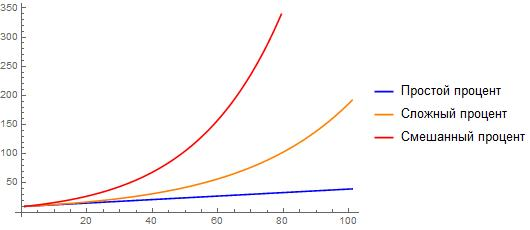
\includegraphics[scale=0.6]{images/first.jpg}
	\caption{График простой, сложной и процентной ставки}
	\end{center}
\end{figure}

% Билет 8 23.59 15.06.2020

\subsection{Связь между простыми и сложными ставками }

\begin{definition}
	Процентные ставки являются \textit{финансово эквивалентными}, если замена в контракте одной ставки на другую не приводит к изменению финансовых результатов контракта, к изменению отношений участвующих в сделке сторон.
\end{definition}

Если рост по простой процентной ставке за определенное время приводит к тому же результату, что и рост по сложной процентной ставке за то же время, то эти ставки финансово эквивалентны.

Пусть $i_n$ и $i_c$ - простая и сложная процентные ставки c одним и тем же периодоим начисления (например, годовые ставки). Приравняем множители роста по этим ставкам за время $t$:
$$1 + i_n \cdot t = (1 + i_c)^t$$

Отсюда можно получить формулы, позволяющие по сложной ставке рассчитать эквивалентную ей простую и по простой ставке определить эквивалентную ей сложную:
$$i_n = \frac{(1 + i_c)^t - 1}{t}$$
$$i_c = \sqrt[t]{1+i_n \cdot t} - 1$$

Отметим, что при изменении длины промежутка, меняется и величина экивалентной ставки.

При $t=1$, то есть когда длина рассматриваемого промежутка равна периоду начисления, эквивалентные ставки равны друг другу:
$$i_n = i_c$$

Как показывают предыдущие рассуждения:
$$t<1 \Leftrightarrow i_n < i_c$$
$$t>1 \Leftrightarrow i_n > i_c$$

\subsubsection{Задача о.в Манхэттен}
\label{second_table}
\begin{table}[H]
	\begin{center}
		\begin{tabular}{c|c} 
		t (год) & Деньги (\$) \\ \hline
		$t_1$ - 1626 год & $P - 24$ \\ \hline
		$t_2$ - 2019 год & $S - 49\cdot 10^9$
		\end{tabular}
		\caption{Данные о Манхэттене}
	\end{center}
\end{table}

\textbf{Вопрос}: Какова процентная ставка при простом и сложном проценте?

\textbf{Решение:}

Простой процент: 
$$i=\frac{\frac{S}{P}-1}{t}=\frac{S-P}{(t_2-t_1)\cdot P}=\frac{49\cdot 10^9-24}{24*(2019-1626)}=5.19 \cdot 10^6$$

Сложный процент: 
$$i=\sqrt[(t_2-t_1)]{\frac{S}{P}}-1=\sqrt[2019-1626]{\frac{49\cdot 10^9}{24}}-1 = 0.056 = 5.6\%$$

Срок удвоения оклада: 
$$t_{new}=log_{(1+i)} 2 = log_{(1+0.056)} 2 = 12.7 \approx 13 \text{ years}$$ 

% Билет 11. 0.46 16.06.2020

\subsection{Сложная переменная ставка}

В некоторых случаях может быть оговорена переменная ставка. Связано это может быть с процессом инфляции.

Рассмотрим ситуацию с переменной сложной процентной ставкой. Пусть на первом промежутке времени длиной $t_1$ ставка равна $i_1$, на втором промежутке $t_2$ ставка равна $i_2$ и.т.д.

Промежутки, как и раньше, имеют различную длину.

Рассмотрим $n$ таких промежутков длиной $t_1,t_2,\ldots,t_n$. Величина конечного вклада по сложной переменной ставке к концу последнего промежутка составит:
$$S = P \cdot (1+i_1)^{t_1} \cdot (1+i_2)^{t_2} \cdot \ldots \cdot(1+i_n)^{t_n} = P \prod\limits_k^n (1+i_k)^{t_k}$$

Определим среднюю процентную ставку $i$ для случая вклада по сложной переменной ставке.

\begin{proof}
	Обозначим за $T$ - общий срок вклада по переменной ставке.
	$$ T =  \sum_{i}{t_i} $$
	а посредством $\tau_i$ - долю промежутка $t_i$ в общем сроке:
	$$\tau_i = \frac{t_i}{T}, \qquad \sum_i \tau_i = 1 $$

	Средняя процентная ставка удовлетворяет условию, что если ее подставить в формулу роста вместо каждой из ставок $i_k$, то результат расчета при этом не изменится. Таким образом, формула для конечного вклада при переменной ставке для сложных процентов:
	$$ S = P \cdot (1+i_1)^{t_1} \cdot (1+i_2)^{t_2} \cdot \ldots \cdot(1+i_n)^{t_n} = P\cdot (1+ \overline{i})^T$$
	$$ (1+\overline{i})^T =  (1+i_1)^{t_1} \cdot (1+i_2)^{t_2} \cdot\ldots \cdot(1+i_n)^{t_n}$$

	Откуда переменная сложная процентная ставка равна:
	$$ \overline{i} = (1+i_1)^{\tau_1} \cdot (1+i_2)^{\tau_2} \cdot \ldots \cdot(1+i_n)^{\tau_n} - 1 =  \prod_k^n (1+i_k)^{\tau_k}  - 1$$

	В частном случае, когда длины всех промежутков времени равны друг другу, доля каждого из них равна $\frac{1}{n}$ и средневзвешенная величина перходит в обычную среднегеометрическую:
	$$1+ \overline{i} =  \sqrt[n]{(1+i_1)\cdot (1+i_2)\ldots \cdot(1+i_n)}$$
\end{proof}

% Билет 6

\subsection{Характеристики роста по простым и сложным процентам}

Рассмотрим рост величины вклада по формулам простых и сложных процентов при одной и той же величине процентной ставки.

Пусть начисление процентов идет по ставке $i$ за период времени (например, год). Тогда рост суммы за время $t$ от начальной величины $P$ определяется следующими формулами.

Для простых процентов: $S = P(1+it)$

Для сложных процентов: $S = P(1+i)^t$

Для простых процентов величина $S$ зависит от времени $t$ по закону линейной функции, а для сложных - по закону показательной.

Рассмотрим график зависимости простой и сложной ставки.

\begin{center}
	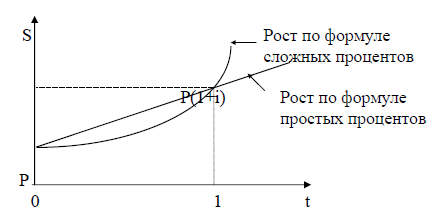
\includegraphics[scale=0.8]{images/a1.png}
\end{center}

Обе линии на рисунке начинаются в одной точке. При $t=0$:
$$S = P\cdot (1+i \cdot 0) = P\cdot (1+i)^0 = P$$

Если длина промежутка времени $t$ меньше длины периода, то простые проценты дают больший рост суммы, чем сложные.

Если $0 < t < 1$, то:
$$P(1+it) > P(1+i)^t$$

Если промежуток времени $t$ равен одному периоду, то расчет по простым и сложным процентам дает один и тот же результат:
$$S = P(1+i\cdot 1) = P(1+i)^{1} = P(1+i)$$

Оба графика проходят через одну точку. 

Если же длина промежутка $t$ больше одного периода, то сложные проценты дают больший рост суммы, чем простые. Если $t > 1$, то:
$$P(1+it) < P(1+i)^t$$

График показательной функции лежит выше прямой, причем с ростом $t$ увеличивается не только величина расхождения между ними, но и скорость увеличения этого расхождения. Если срок вклада больше периода начисления прцентов, то вклакдчику вгыоднее начисления по формуле сложных процентов, причем с ростом строка вклада эта выгода возрастает.

% Билет 9. 0.28 16.06.2020

\subsection{Формулы срока удвоения}

Для оценки скорости роста денежной суммы часто используют так называемые \textbf{формулы срока удвоения}. Такие формулы позволяют рассчитать срок $t_d$, за который \textit{удваивается вложенная сумма денег.}

Такой срок рассчитвыется путем решения уравнения, определяющего удвоение коэффициента нарастания.

Для простых процентов получаем, что:
$$S = 2P = P \cdot (1 + i \cdot t_{d})$$
$$t_d = \frac{1}{i}$$

Для сложных процентов уравнение имеет вид:
$$S = 2P = P \cdot (1+i)^{t_d}, \Leftrightarrow (1+i)^{t_d} = 2$$
$$t_d = \log_{1+i} 2 $$

% Билет 10 0.36 16.06.2020


\subsection{Непрерывный рост суммы и сила роста}

В банковской практике часто используется смешанная форма перевода процентных ставок, при котором сложная годовая ставка переводится, в квартальную как простая. Дальнейшее же начисление процентов идет по формуле сложной ставки.

Допустим, что банк предъявляет условия вклада как $48 \%$ годовую ставку с ежеквартальным начислением процентов.

Это означает, что проценты ежеквартально приплюсовываются к уже накопленной величине вклада и на них в дальнейшем начисляются проценты. Речь таким образом идет о сложной ставке.

Однако сами квартальные проценты расчитываются по формуле простой ставки, то есть:
$$i_{\text{кв}} = \frac{i_{\text{год}}}{4} = 12\%$$

В обратном переводе в сложную годовую ставку это дает:
$$(1+i_{\text{кв}})^4 \approx 1,57$$
то есть $57$ процентов годовых вместо $48 \%$. Результат всегда оказывается завышенным и банку невыгоден результат, а клиенту выгоден.

Если уменьшать период, то процент будет увеличиваться.

Допустим, что период начисления уменьшается дальше, то есть год дробится на $m$ одинаковых промежутков времени и величина $m$ растет. Тогда общая формула нового коэффициента годового роста выглядит следующим образом:
$$\left(1+\frac{i}{m}\right)^m, i > 0, t >1$$

При этом рост единицы вклада за время $t$ определяется формулой в пределе:
$$\lim\limits_{m \to \infty} \left(1+\frac{i}{m}\right)^{tm} = \lim\limits_{m \to \infty} \left(\left(1+\frac{i}{m}\right)^{\frac{m}{i}}\right)^{ti} = e^{it}$$

Таким образом, рост вклада есть величина:
$$S = P \cdot e^{it}$$

\begin{definition}
	Начисление процентов таким образом называется \textit{непрерывным}.

	Мы пришли к понятию непрерывных процентов через смешанную форму начисления, через соединение расчетов по простой и сложной ставке. Однако смешанная форма не важна, существенно лишь участие сложной ставки.
\end{definition}
Формулу сложных процентов для непрерывного времени преобразуют таким образом, чтобы при разных ставках основание оказывалось одинаковым, а изменялся бы показатель степени.

От понятия сложной ставки к понятию непрерывных процентов можно перейти следующим путем:
$$S = P(1+i)^t = P\cdot e^{\alpha t}$$
где $\alpha = \ln {1+i}$. Эта фомула используется при анализе непрерывного роста суммы денег.

В этой формуле величина $\alpha$ характерищует скорость роста суммы.

\begin{definition}
	Величину $\alpha$ называют \textit{силой роста} или \textit{силой процента}. Она равна скорости относительного прироста суммы, то есть равна относительному приросту суммы за бесконечно малый промежуток времени.
\end{definition}
\begin{proof}
Покажем это:
$$S(t) = P \cdot e^{\alpha t}$$

Высчитаем силу прироста для функции $S(t)$:
$$\frac{\Delta S(t)}{S \cdot \Delta t}\underset{t \to 0}{=}\frac{S'}{S} = \frac{P \cdot e^{\alpha t} \cdot \alpha}{P \cdot e^{\alpha t}} = \alpha$$
\end{proof}

% Билет 12 1.26 16.05.2020


\subsection{Расчёт величины сложной процентной ставки}

Формула для процентной ставки: $$i=\sqrt[t]{\frac{S}{P}}-1$$

Пусть период начисления по процентной ставке $i$ делится на $m$ одинаковых промежутков времени. Тогда процентная ставка $i'$, связанная с этими промежутками, определеяется через ставку $i$ в соответствии с соотношением:
$$(1+i')^m = 1+i$$

Отсюда:
$$i' = \sqrt[m]{1+i} - 1$$
$$i' = \sqrt[m]{1+\sqrt[t]{\frac{S}{P}}-1}-1 = \sqrt[mt]{\frac{S}{P}} - 1$$

Второй способ:
$$S = P \cdot (1+i')^{mt}$$
$$i' = \sqrt[mt]{\frac{S}{P}} - 1$$

Рассмотрим теперь непрерывное начисление процентов на основе силы роста. В этом случае формула нарастания имеет вид:
$$S = Pe^{\alpha t}$$

Отсюда получаем расчетную формулу для определения силы роста (непрерывной ставки процента) $\alpha$:
$$\alpha = \frac{\ln \frac{S}{P}}{t}$$

% Билет 13 1.40 16.05.2020

\subsection{Расчёт продолжительности срока по сложным процентным ставкам }

Формула для продолжительности вклада:
$$ t = \log_{1+i}\left({\frac{S}{P}}\right)$$

Эта формула позволяет по заданной начальной и конечной сумме и при известной ставвке сложного проценат определить продолжительность того срока $t$, за который начальная сумма $P$ вырастет до конечной суммы $S$ по ставке сложного процента $i$.

Пусть период начисления по процентной ставке $i$ делится на $m$ одинаковых промежутков времени. Тогда процентная ставка $i'$, связанная с этими промежутками, определеяется через ставку $i$ в соответствии с соотношением:
$$(1+i')^m = 1+i$$

Отсюда:
$$i' = \sqrt[m]{1+i} - 1$$

Рост денежной суммы за время $t$ по ставке $i'$ будет идти в соответствии с формулой:
$$S = P \cdot (1+i')^{mt}$$
$$t = \frac{\log_{1+i'} \left({\frac{S}{P}}\right)}{m}$$

При расчетах на основе силы роста используют формулу:
$$S = P\cdot e^{\alpha t}, \Leftrightarrow t = \frac{\ln {\left(\frac{S}{P}\right)}}{\alpha} =  \frac{\ln {\left(\frac{S}{P}\right)}}{\ln{1+i}} $$

% Билет 14 1.48 16.05.2020


\newpage
\section{Консолидация и конверсия}

\subsection{Консолидация платежей}

Предположим, что одно лицо брало несколько раз ссуду у другого лица и теперь должно вернуть ему определенные суммы денег в различные моменты времени. По договоренности обеих сторон может быть произведена \textit{консолидация}, то есть объединение этих нескольких платежей в один платеж. 

Следует определить \textbf{срок возврата} консолидируемой суммы и \textbf{размер этой суммы}. В этом состоит задача консолидации платежей.

Интересы сторон обычно оказываются противоположными. Одна сторона хочет вернуть деньги позже и в меньшем объеме, в то время как другая желает получить их раньше и в большей сумме. Следует найти справедливое решение, которое устроило бы обе стороны.

Справедливое решение соответствует принципу финансовой эквивалентности платежей. То есть пусть имеется $n$ платежей, соответствующих различным суммаи и приуроченных к различным моментам времени. Такие платежи считаются финансово эквивалентными, если они будучи приведенными по заданной ставке процента к одному моменту времени, оказываются равными.

\begin{definition}
	\textit{Решение задачи консолидации нескольких платежей} - это определение такого размера единого платежа и такого момента его выплаты, которые финансово эквивалентны всей заменяемой совокупности платежей. 
\end{definition}

Пусть платежи имеют размеры $S_1, S_2,\ldots, S_m$ и они должны быть выплачены в соответствующие моменты времени $t_1,t_2,\ldots,t_m: t_1 < t_2 < \ldots < t_m$.

Предположим, что всю эту совокупность платежей следует консолидировать, то есть заменить одним платежом размера $S$. Следует определить справедливый момент выплаты $t$ этого платежа.

Мы рассмотрим задачу в предположении, что величина консолидированного платежа $S$ равна сумме консолидируемых платежей:
$$S = \sum\limits_{k=1}^m S_k$$

Искомый момент времени $t$ выплаты консолидированной суммы $S$ не может наступить ранее срока первого платежа или в сам момент $t_1$, на это не согласиться сторона, которая должна выплачивать платежи, потому что в более ранний срок нужно выплатить ту же сумму $S$.

Искомый момент $t$ не может наступить и позже срока последнего платежа $t_m$ или в сам момент $t_m$. На это не пойдет та сторона, которая должна получать платежи. Она могла бы на это согласиться, если бы консолидированная величина была больше суммы консолидируемых платежей. Однако по предположению они равны друг другу. Таким образом, $ t < t_m $.

Итак, искомый момент $t$ лежит в промежутке от $t_1$ до $t_m$. Для части консолидируемых платежей моменты их выплаты окажутся раньше, чем $t$. Такие платежи назовем \textit{ранними платежами}. 

Моменты выплаты другой части платежей окажутся позже, чем $t$. Эти платежи назовем \textit{поздними платежами}.

С точки зрения уплачивающей стороны при консолидации она проигрывает по поздним платежам (так как их при консолидации придется выплатить раньше), но выигрывает по ранним платежам (их при консолидации следует уплатить позже). С точки зрения получающей стороны все наоборот, она проигрывает по ранним платежам, но выигрывает по поздним. То, что проигрывает одна сторона, выигрывает другая.

Консолидация будет справедливой, если для каждой из сторон суммарный выигрыш будет равен суммарному проигрышу. При этом достаточно уравновесить выигрыш и проигрыш для одной стороны. Отсюда будет следовать, что они уравновешены и для другой.

\subsection{Определение времени уплаты консолидированной суммы}

\subsubsection{Простая процентная ставка}

Будем использовать простую процентную ставку $i$.

До консолидации уплачивающая сторона должна была выплатить платеж $S_1$ в момент $t_1$. В результате она выплатит платеж, но в более поздний момент $t$.

За промежуток времени от $t_1 \to t$ величина по ставке $i$ могла бы вырасти на величину $L_1$:
$$L_1 = S_1 \cdot i \cdot (t-t_1)$$

Это величина - выигрыш уплачивающей стороны, связанный с переносом на более поздний срок.

Проведем рассуждение для всех ранних платежей:
$$L_p = S_p \cdot i (t-t_p)$$

Общий выигрыш равен сумме выишрышей при консолидации по всем ранним платежам:
$$L = \sum\limits_p L_p = \sum\limits_p S_p \cdot i \cdot (t-t_p)$$

Поздние платежи связаны с проигрышем при консолидации для уплачивающей стороны, поскольку их выплачивать придется в том же объеме, но ранше по сроку.
$$R = \sum\limits_q R_q = \sum\limits_q S_q \cdot i \cdot (t_q-t)$$

Условие финансовой эквивалентности, справедливости замены сроков платежей при их консолидации означает, что общий выигрыш и общий проигрыш равны:
$$L=R, \Leftrightarrow  \sum\limits_p S_p \cdot i \cdot (t-t_p) = \sum\limits_q S_q \cdot i \cdot (t_q-t)$$

Если один из платежей оказался на границе, то соответствующие ему выигрыш и проигрыш равна $0$.
$$ \sum\limits_p S_p \cdot (t-t_p) -  \sum\limits_q S_q \cdot (t_q-t) = 0$$
$$ \sum\limits_p S_p \cdot (t-t_p) +  \sum\limits_q S_q \cdot (t-t_q) = 0$$
$$\sum\limits_{k=1}^m S_k(t-t_k) = 0$$
$$\sum\limits_{k=1}^m S_k\cdot t - \sum\limits_{k=1}^m S_k t_k = 0$$
$$tS = \sum\limits_{k=1}^m S_k t_k$$
$$t = \frac{\sum\limits_{k=1}^m S_k t_k}{S} = \sum\limits_{k=1}^m \frac{S_k}{S} t_k$$
Обозначая за $\alpha_k = \frac{S_k}{S}$, получим:
$$t = \sum\limits_{k=1}^m \alpha_k t_k$$

Таким образом момент $t$ уплаты консолидированной суммы $S$ равен сумме моментов внесения $t_k$ отдельных платежей, в этой сумме каждый $t_k$ берется с коэффициентом, равным той доле, которую составяет данный платеж $S_k$ в общей консолидированной сумме $S$.

\subsubsection{Сложная процентная ставка}

Пусть объединяются $m$ платежей, имеющих суммы $S_1,S_2,\ldots,S_m$ и сроки $t_1,t_2,\ldots,t_m$. Предположим, что сумма общего платежа равна $S$. Требуется определитель срок общего платежа $t$.

Если все платежи привести к моменту времени $t$ по процентной ставке $i$, то получим равенство:
$$\sum_{k=1}^{n} p_k (1+i)^{(t^*-t_k)} = S (1+i)^{(t'-t^*)}$$
$$\sum_{k} p_k (1+i)^{t'} (1+i)^{-t_k} = (1+i)^{t'}\sum_{k} (1+i)^{-t_k} = (1+i)^{t'}\frac{S }{(1+i)^{t^*}}$$
$$\sum\limits_{k=1}^m S_k (1+i)^{t-t_k} = S$$
$$(1+i)^{t} = \frac{S}{\sum\limits_{k=1}^{n} S_k (1+i)^{-t_k} }$$
$$t = \log_{1+i} \frac{S}{\sum\limits_{k=1}^{n} S_k (1+i)^{-t_k} } = \log_{1+i} (S) - \log_{1+i} \left(\sum\limits_{k=1}^{n} S_k (1+i)^{-t_k} \right)$$
$$t = - \log_{1+i} \sum\limits_{k=1}^{n} \frac{S_k}{S} (1+i)^{-t_k}  = - \log_{1+i} \frac{\sum S_k (1+i)^{-t_k/365}}{S} \cdot 365$$

% Билет 16 / 35 16.06.2020

\subsection{Консолидация платежей с изменением срока выплаты или уплачиваемой суммы}

Мы рассмотрели задачи объединения и разъединения платежей без изменения их общей суммы. На практике встречаются и другие задачи, когда изменяется общая сумма платежей или срок выплаты.

Пусть несколько платежей $S_1,S_2,\ldots,S_m$ консолидируются в один платеж $S$, по величине равный сумме этих отдельных платежей:
$$S = \sum\limits_{k=1}^m S_k$$

Момент выплаты $t$ консолидированной суммы:
$$t = \sum\limits_{k=1}^m \frac{S_k}{S} \cdot t_k$$
Пусть по условию договора изменяется срок уплаты общей суммы платежей. Вместо момента времени $t$ платеж будет произведен позже, в момент $t'$. Тогда изменится и выплачиваемая сумма и нам следует выплатить большую сумму $S'$.

Величина $S'$ должна быть определена в соответствии с принципом финансовой эквивалентности.

$\Delta t = t' - t$ - разность между новым и старым моментом выплаты. За время сумма $S$ должна вырасти по формуле простых процентов и достичь величины $S'$:
$$S' = S(1+i\cdot \Delta t)$$

Это и есть искомая величина выплаты в момент $t'$. При переносе на ранний срок, $\Delta t$ будет отрицательной  и новая сумма $S'$ будет меньше исходной суммы $S$.

Обратная задача: нахождение срока изменения суммы.

Пусть по условиям договора вместо прежней суммы $S$ следует уплатить $S'$. Следует определить $t'$ этой суммы.
$$\Delta t = t' - t, \qquad S' = S(1+i\Delta t)$$
$$\Delta t = \frac{\frac{S'}{S} - 1}{i} \quad \Longrightarrow \quad t' = \Delta t + t = t + \frac{\frac{S'}{S} - 1}{i}$$

% Билет 17/35 15.14 16.05.2020

\subsection{Расчёты с конверсией валют по простым процентным ставкам }

Рассмотрим расчет оценок доходности, связанных с возможностью замены валюты.

Пусть имеется возможность перевода вклада из валюты $1$ (рубли) в валюту $2$ (доллары). Введем параметры вклада.

\begin{itemize}
	\item $P_1$ - исходная суммая средств в валюте $1$
	\item $P_2$ - та же сумма средств в валюте $2$
	\item $i_1$ - процентная ставка по вкладу в валюте $1$
	\item $i_2$ - процентная ставка по вкладу в валюте $2$
	\item $t$ - срок вклада
	\item $S_1$ - конечная сумма средств в валюте $1$
	\item $S_2$ - конечная суммая средств в валюте $2$
	\item $S_1'$ - сумма средств, накопленная в валюте $2$ и переведенная в валюту $1$
	\item $K_{12}$ - начальный курс валюты $2$ относительно валюты $1$
	\item $K_{12}(t)$ - курс валюты $2$ относительно валюты $1$ к концу срока $t$. $K_{12} = K_{12}(0)$
\end{itemize}

Вкладчик имеет сумму средств $P_1$ в валюте $1$. К концу срока он получит:
$$S_1 = P_1 \cdot (1+i_1 \cdot t)$$

Вторая возможность - перевести деньги в валюту $2$ и затме использовать вклад в валюте $2$. В результате перевода ваюты он получит сумму $P_2$:
$$P_2 = \frac{P_1}{K_{12}}$$

К концу срока $t$ он получит $S_2$:
$$S_2 =  P_2 \cdot (1+i_2 \cdot t) = \frac{P_1 \cdot (1+i_2 t)}{K_{12}}$$

Для сопоставления результатов их следует привести в одну валюту. Пусть это валюта $1$. Сумма $S_2$ конвертируется в сумму $S_1'$ по формуле:
$$S_1' = S_2 \cdot K_{12}(t) = \frac{P_1 \cdot (1+i_2 t)}{K_{12}} \cdot K_{12}(t) $$

Между собой нужно сравнить $S_1$ и $S_1'$ - что выгоднее?

При принятии решения необходимо спрогнозировать курс $K_{12}(t)$. Предположим, что у нас линейная функция:
$$K_{12}(t) = K_{12} \cdot (1 + kt)$$
где $k$ - средняя величина прироста валютного курса за единицу времени. Величина прироста $k$ может быть положительной (курс валюты $2$ в среднем растет) или отрицательной (курс валюты $2$ в среднем падает).
$$\frac{P_1}{K_{12}} \cdot (1 + i_2 t) \cdot K_{12}(t) = \frac{P_1}{K_{12}} \cdot (1 + i_2 t) \cdot K_{12} (1 + kt) = P_1 \cdot (1 + i_2 t) (1 + kt)$$
$$S_1' - S_1 = P_1 \cdot (1 + i_2 t) (1 + kt) - P_1 \cdot (1+i_1 \cdot t) = P_1(i_2kt^2 + (k+i_2-i_1)t)$$
Полезной для анализа является величина разности, приходящейся на вклад единичной величины при $P_1=1$. То есть:
$$S_1' - S_1 = i_2kt^2 + (k+i_2-i_1)t$$

1. Предположим, что $k >0$. Найдем условие крайности:
$$i_2kt^2 + (k+i_2-i_1)t = 0$$
Корни того уравнения:
$$t_1=0 \qquad t_2=\frac{i_1-i_2-k}{i_2k}$$

Если $t_2 \leq 0$, то есть если $i_1 \leq i_2+k$, то вариант с конверсией валюты $1$ в валюту $2$ дает больший результат ри любом сроке вклада $t$.

Есди $t_2 >0$, то есть если $i_1 >i_2+k$, то вариант с конверсией валюты дает больший результат лишь результат лишь при достаточно большом сроке вклада $t$, а именно при $t > t_2$.

То есть, если $i_1 >i_2+k$, то вариант с конверсией валюты дает больший результат лишь результат лишь при достаточно большом сроке вклада $t$. Иначе - вариант с конверсией валюты 1 в валюту 2 дает болший результат при любом сроке.

\textbf{Вывод:} конверсионный вариант выгоднее, если срок вклада $t$ больше большей из двух величин $t_1$ и $t_2$, то есть если:
$$t > \max\left\{0,\frac{i_1-i_2-k}{i_2k}\right\}$$

2. $k < 0$

В этом случае коэффициент $i_2k$ отрицателен. Квадратичная функция убывает. Вклад, связанный с конверсией валюты, со временем станет менее выгодным, чем вклад без конверсии.

% Билет 18  15.44 16.05.2020

\subsection{Расчёты с конверсией валют по сложным процентным ставкам }

Рассмотрим теперь сложные процентные ставки.

Конечная величина вклада без конверсии валюты:
$$S_1 = P_1 \cdot (1+i_1)^t$$

Конечная величина вклада с конверсией валюты $1$ в валюту $2$ в начале срока и обратной конверсией по окончанию срока определяется фомрулой:
$$S_1' = S_2 \cdot K_{12}(t) = \frac{P_1 \cdot (1+i_2)^t \cdot K_{12}(t)}{K_{12}}$$
Рассмотрим новую форму прогноза валютного курса:
$$K_{12}(t) = K_{12} \cdot (1+k)^t$$
где $k$ - относительный прирост курса. Сама величина $k$ может быль положительной (курс валюты $2$ растет) или отрицательной (курс валюты $2$ падает).
$$\frac{S_1'}{S_1} = \frac{\frac{P_1 \cdot (1+i_2)^t \cdot K_{12}(t)}{K_{12}}}{P_1 \cdot (1+i_1)^t} = \left(\frac{(1+i_2)(1+k)}{1+i_1}\right)^t$$

Вклад с конверсией будет выгоднее бесконверсионного вклада, если:
$$(1+i_2) \cdot (1+k) > 1+i_1, \Leftrightarrow k > \frac{i_1-i_2}{1+i_2}$$
$k$ характеризует ограничение снизу на темп роста валютного курса.

Если неравенство выполнено, то есть темп роста валютного курса высок, то выгоден конверсионный вариант. Если же обратное, то выгоден конверсионный вариант.

При
$$k = \frac{i_1-i_2}{1+i_2}$$
оба вариванта равносильны.

\subsubsection{Приведение платежей}
Для простой процентной ставки:
$$ P_2 = P_1 \cdot (1 + i (t_2-t_1)), \text{если } t_2 > t_1 $$
$$ P_2 = \frac {P_1}{(1+i(t_1-t_2))}, \text{если } t_2 < t_1 $$
$$ P_3 = P_1 (1+i(t_2-t_1)) \cdot (1+i(t_3-t_2)) \neq P_1 (1+i(t_3-t_2))$$

Для сложной процентной ставки:
$$ P_2 = P_1 \cdot (1 + i)^{(t_2-t_1)}, \text{если } t_2 > t_1 $$
$$ P_2 = \frac{P_1}{(1+i)^{(t_1-t_2)}} = P_1 \cdot (1 + i)^{(t_2-t_1)}, \text{если } t_2 < t_1$$
$$ P_3 =P_1 \cdot (1 + i)^{(t_2-t_1)} \cdot (1 + i)^{(t_3-t_2)} = P_1 (1+i)^{(t_3-t_1)}, \text{если } t_2 < t_1$$

% Билет 19 15.53 16.05.2020

\subsection{Расчёт среднего темпа инфляции }

Обычные формулы расчетов позволяют расчитать номинальный рост денежной суммы. В связи с инфляцей - чрезмерного увеличения количества обращающихся в стране бумажных денег - сумма может постепенно обесцениваться. 

Поэтому следует учиывать характеристики инфляции.

\begin{definition}
	\textit{Индекс инфляции} - показывает, во сколько раз изменился уровень цен за анализируемый период.
\end{definition}
\begin{definition}
	\textit{Темм инфляции}  - характеризует прирост уровня цен.
\end{definition}

Темпы показывают инфляционный прирост уровня цен на конце данного месяца по отношению к концу предыдущего месяца.

Для определения прироста уровня цен по отношению к базе - началу года - следует преобразовать цепные темпы в базовые.

\textbf{Цепной индекс}  - цепной темп $+1$.

\textbf{Базовый индекс} - последовательное перемножене цепных индексов на определенный месяц.

\textbf{Базовый темп инфляции} -  базовый индекс $-1$.

\textbf{Средний индекс инфляции} - корень $n$-ой степени из произведения цепных индексов.

\textbf{Средний месячный индекс} - корень $n$-ой степени из произведения цепных индексов.

% Билет 20/35 16.18 16.05.2020

\subsection{Учёт инфляции в одном периоде времени, реальная процентная ставка}

Пусть денежный вклад растет по процентной ставке $i$. Тогда коэффициент роста в течение одного периода  - $1+i$ для простой и сложной процентной ставке.

Предположим, что из-за инфляции происходит обесценивание денег. Тем инфляции за этот промежуток обозначим за $h$.

Таким образом, реальная оценка денежного вклада изменяется одновременно под воздействием двух разнонаправленных факторов: номинальная сумма растет по условию вклада, а под влияением инфляции его покупательная способность падает.

\textbf{Формулы Фишера}

\begin{definition}
	\textit{Реальная процентная ставка $r$} - характеризует реальную оценку роста.
\end{definition}

\begin{definition}
	\textit{Коэффициент реального роста} вклада $1+r$ определяется по формуле:
	$$1 + r = \frac{1+i}{1+h}$$

	Следовательно, реальная процентная ставка:
	$$r = \frac{i-h}{i+h}$$
	где $i$ - номинальная процентная ставка (\textit{ставка-брутто}), а $r$ - реальная процентная ставка (\textit{ставка-нетто}).
\end{definition}
$$R = P(1+r) = P \cdot \frac{1+i}{1+h}$$ - новая стоимость первоначального вклада с учетом инфляции.

% Билет 21/35 16.27 16.05.2020

\subsection{Учёт инфляции в нескольких периодах времени}

Рассмотрим теперь влияние инфляции в течение нескольких периодов.

Пусть в течение $n$ периодов темпы инфляции были равны величинам $h_1,\ldots,h_n$.

1. \textbf{Простая процентная ставка.}

Тогда коэффициент реального роста вклада за время $1+r \times n$ определяется формулой:
$$1 + r \cdot n = \frac{1+i\cdot n}{(1+h_1)\cdot \ldots \cdot (1+h_n)}$$ 

Откуда находим величину реальной простой процентной ставки $r$:
$$r = \frac{\frac{1}{n} + i}{(1+h_1)\cdot \ldots \cdot (1+h_n)} - \frac{1}{n}$$ 

2. \textbf{Сложная процентная ставка.}

Тогда коэффициенты реального роста вклада за время $(1+r)^n$ определяются формулой:
$$(1+r)^n = \frac{(1+i)^n}{(1+h_1)\cdot \ldots \cdot (1+h_n)}$$

Отсюда находим среднюю величину коэффициента реального роста:
$$1 + r = \frac{1+i}{\sqrt[n]{(1+h_1)\cdot \ldots \cdot (1+h_n)}}$$

Средняя величина реальной сложной процентной ставки:
$$r = \frac{1+i}{\sqrt[n]{(1+h_1)\cdot \ldots \cdot (1+h_n)}} - 1$$

Числитель - коэффициент роста за период, знаменатель - средний индекс инфляции.

% Билет 22/35 16.35 16.05.2020

\newpage
\section{Характеристики потоков платежей}

Операции с отдельными денежными суммами лежат в основе более сложных операций - операций с последовательностями таких сумм, распределенных во времени, то есть с потоками платежей. 

\begin{definition}
\textit{Потоком платежей} называется последовательность денежных сумм, приуроченных к определенным моментам времени. Отдельные денежные суммы, являющиеся членами последовательности, называются \textit{членами потока}.
\end{definition}

Потоки платежей классифицируют на \textbf{регулярные} и \textbf{нерегулярные}.

\begin{definition}
	В \textit{нерегулярном потоке} временные интервалы между членами потока могут иметь \textit{различную продолжительность}.

	Кроме того, члены такого потока могут иметь различные знаки. Положительные члены обычно соответствуют поступлениям денежных сумм, отрицательные – затратам.
\end{definition}

\begin{definition}
	В \textit{регулярном потоке} промежутки времени между соседними выплатами имеют \textit{одинаковую длину} и члены потока имеют один знак. Регулярные потоки называются также \textit{финансовыми рентами}.
\end{definition}

Отметим, что члены финансовой ренты в общем случае могут различаться по своей величине. 

Если они одинаковы, то говорят о \textit{постоянной финансовой ренте.} Если различаются - то о \textit{переменной финансовой ренте.} 

К основным параметрам, характеризующим ренту, относятся:
\begin{itemize}
	\item \textbf{член ренты} - размер отдельного платежа
	\item \textbf{период ренты} - длина интервала времени между соседними платежами
	\item \textbf{срок ренты} - длина промежутка времени от начала первого 
	\item \textbf{процентная ставка} - та величина процентной ставки, на основе которой проводится анализ ренты
\end{itemize}

\begin{definition}
	\textit{Вечная рента} - рента, не имеющая заранее оговоренного срока.
\end{definition}

Ренты различаются по моменту выплат в пределах периода. 

\begin{definition}
	Если платежи приурочены к концу периодов, то рента называется \textit{рентой пост-нумерандо} (а также обыкновенной рентой).
\end{definition}
\begin{definition}
	Если же платежи приурочены к началу периодов, то рента называется \textit{рентой пренумерандо.}
\end{definition}

\subsection{Общие характеристики потоков платежей}

Два финансовых потока могут быть по-разному распределены во времени, иметь различную продолжительность, число членов и.т.д. Их сопоставление, выбор варианта поток проводится на основе обобщающиъ характеристик, позволяющих свести разнообразие потоков к небольшому числу базовых показателей.

К основной характеристике потока относится его приведенная стоимость. Она позволяет свернуть весь потом во времени в одно число. 

\begin{definition}
	\textit{Приведенная стоимость потока} - сумма всех членов потока с начисленными процентами, приведенная (дисконтированная) к какому-то заданному моменту времени. 

	Обычно выбирают либо начало первого периода, либо момент окончания последнего периода. В первом случае говорят о \textit{современной стоимости(оценке)} потока, во втором - о \textit{наращенной стоимости (сумме)} потока. 
\end{definition}

% Билет 23/35 16.58 16.05.2020

\subsection{Расчёт приведённой стоимости потока}

Пусть поток состоит из членов $R_k$, приуроченных к моментам времени $t_k$. Определим стоимость этого потока, приведенную к произвольному моменту времени $t$.

Рассмотрим $R_k$ - произвольный член потока. Если $t_k < t$, то при пересчете оценки величины $R_k$ на момент $t$ ее следует увеличить, умножив на коэффициент роста, равный $(1+i)^{t-t_k}$ - показывает, насколько изменится $R_k$ по сложной процентной ставке $i$ за время $t - t_k$.

Если же $t_k >t$, то формула та же, что и для прежнего коэффициента роста, то есть $(1+i)^{t-t_k}$, однако показатель степени отрицательный, коэффициент меньше $1$ и величина $R_k$ уменьшается при домножении на него.

Т.о, независимо о расположения, при приведении члена потока $R_k$ к моменту $t$ его следует умножить на:
$$(1+i)^{t-t_k}$$

\begin{definition}
	Приведенная стоимость всего потока $S_t$, приведенная на момент времени $t$ по сложной процентной ставке $i$, определяется суммой результатов приведения всех членов потока, то есть формулой:
	$$S_t= \sum_{k} R_k (1+i)^{t-t_k}$$
\end{definition}

Формула позволяет определить приведенную стоимость потока для любого момента времени $t$. В частности, если $t$ - момент начала потока, то эта формула определяет современную стоимость потока. Если же $t$ - момент окончания срока потока, формула определяет наращенную сумму потока.

% Билет 24/35 17.07 16.05.2020

\subsection{Связь между результатами приведения потока к разным моментам времени}

Пусть $t'$ - другой момент приведения. Тогда при приведении к моменту $t'$ получим величину:
$$S_{t'} = \sum_{k} R_k (1+i)^{t'-t_k}$$

Величины $S_t$ и $S_{t'}$ связаны соотношением:
$$S_{t'} = \sum_{k} R_k (1+i)^{t'-t_k} = (1+i)^{t'-t} \cdot \sum_{k} R_k (1+i)^{t-t_k} = (1+i)^{t'-t} \cdot S_t $$
$$\frac{S_{t'}}{S_t} = (1+i)^{t'-t}$$

Следовательно, при приведении к более позднему моменту величина приведенной стоимости окажется больше.

Отношение $\frac{S_{t'}}{S_t}$ выражается величиной, не зависящей от конкректного потока, зависит лишь от разности моментов приведения и выбранной процентной ставки. Это позволяет сравнить различные потоки по их приведенной стоимости безотносительно к выбору конкректного момента приведения.
$$\frac{S_{t'}^1}{S_{t'}^2} = \frac{S_{t}^1 \cdot (1+i)^{t'-t}}{S_{t}^2 \cdot (1+i)^{t'-t}} = \frac{S_{t}^1} {S_{t}^2}$$

Если приведенная стоимость одного потока оказалась в $m$ раз больше приведенной стоимости другого при приведении обоих потоков к какому-то одному моменту времени, то это же соотношение между потоками сохранится и при приведении к любому другому моменту времени.

% Билет 25/35 17.15 16.05.2020

\subsection{Расчёт характеристик постоянной ренты }

Полученная выше формула приведенной стоимости потока пригодна для расчетов с любыми потоками. В некоторых важных частных случаях ее можно заметно упростить. Так, для наиболее распространенного вида потоков - постоянной финансовой ренты - мы получим существенно более простые расчетные формулы. 

Рассмотрим постоянную ренту, содержащую $n$ членов одинаковой величины $R$. Интервал между членами ренты одинаков. Предположим, что он составляет один год (такая рента называется \textit{аннуитетом}). Пусть это рента постнумерандо.

$n$ одинаковых платежей размера $R$. Общий срок - $n$ лет, очередной платеж - в конце года. Первый платеж - в конце первого года, последний - в конце $n$-го года. Конец общего срока ренты совпадает с моментом последнего платежа.

\textbf{Формула наращенной стоимости ренты $S$} 

Определим наращенную стоимость ренты $S$, то есть стоимость ренты на конец ее срока (наращенную стоимость обозначают иногда также посредством \textit{FV – Future Value}).

Последний, $n$-й член ренты при приведении сохраняется без изменения, поскольку момент приведения совпадает с моментом последнего платежа. В результате преобразования он сохраняет свою величину $R$, предпоследний - $R \cdot (1+i)$.
$$ S = R + R(1+i) + R(1+i)^2 + \cdots + R(1+i)^{n-1}$$

По формуле геометрической прогрессии:
$$ S = R \cdot \frac{(1+i)^n - 1 }{1+i-1} = R \cdot \frac{(1+i)^n - 1 }{i} $$

Это и есть формула \textbf{наращенной суммы} постоянной $n$-членной ренты постнумерандо. 

\textbf{Формула современной стоимости ренты $A$}

Обратимся к формуле современной стоимости ренты A, соответствующей приведению к начальному моменту срока ренты (такую величину обозначают также посредством PV – Present Value). Эту формулу можно получить двумя способами.

Один - провести рассуждения, аналогичные данным выше для формулы наращенной суммы, но ориентированные на приведение к другому моменту времени. 
$$ A = R (1+i)^{-1} + \ldots + R (1+i)^{-n}$$ 
$$ A = \frac{R}{1+i} \cdot \frac{\left(\frac{1}{1+i}\right)^n - 1}{\left(\frac{1}{1+i}\right)-1} = R \cdot \frac {1-(1+i)^{-n}}{i}$$

Другой - провести дисконтирование уже полученной величины наращенной суммы к начальному моменту срока ренты, то есть воспользоваться равенством:
$$ A  = S\cdot (1+i)^{-n}$$
$$ A = R \cdot \frac{(1+i)^n - 1 }{i} (1+i)^{-n} = R \cdot \frac {1-(1+i)^{-n}}{i}$$

% Билет 26/35 17.32 16.05.2020

\subsection{Вечная рента}

В некоторых случаях ренту можно рассматривать как продолжающуюся неограниченно долго, то есть имеющую неограниченное число членов. 

\begin{definition}
	Ренты с неограниченным сроком называются \textbf{вечными рентами.}
\end{definition}

Наращенную сумму определить невозможно, так как такая сумма должна быть приведена к концу срока ренты. Но можно найти современную стоимость вечной ренты:
$$A = \sum\limits_{k=1}^{\infty} R \cdot (1+i)^{-k} = \frac{R}{1+i-1} = \frac{R}{i}$$

Таким образом, современная стоимость вечной ренты определяется простым правилом: современная стоимость равна отношению величины члена ренты к процентной ставке.

Стоимость вечной ренты обратно пропорциональна процентной ставке. При ставке, стремящейся к нулю, современная стоимость вечной ренты стремится к $+\infty$.

% Билет 27/35 17.42 16.05.2020

\subsection{Связь параметров ренты }

Формула наращенной суммы $S$:
$$ S = R \cdot \frac{(1+i)^n - 1 }{i} $$

Формула современной стоимости ренты $A$:
$$A = R \cdot \frac {1-(1+i)^{-n}}{i}$$

Выведем остальные характеристики через эти формулы.

Формула постоянного члена $R$:
$$ R = S \cdot \frac{i}{(1+i)^n - 1}$$
$$ R = A \cdot \frac {i}{1-(1+i)^{-n}}$$

Формула срока ренты $n$
$$ n = \ln_{1+i} \left(\frac{S \cdot i}{R} + 1 \right)$$
$$ n = -\ln_{1+i} \left(1 - \frac{A \cdot i}{R}  \right)$$

В отличии от $R$ и $n$ расчет процентной ставки $i$ не удается провести в виде вычисления по готовой формуле. Величину процентной ставки определяют одним из методов приближенных вычислений.

% Билет 28/35 17.45 16.05.2020

\subsection{Ренты пренумерандо и постнумерандо}

Для ренты постнумерандо FV - последний из периодов, PV - начальная точка. Для ренты преднумерандо PV - вторая точка, FV - точка за последней.

Рента пренумерандо при приведении к концу срока отличается от ренты постнумерандо сдвигом на один период времени от конца назад. Поэтому все ее члены при приведении следует дополнительно умножить на одну и ту же величину $(1 + i)$. В результате формула наращенной суммы ренты пренумерандо примет вид:
$$S_{pre} = R \cdot \frac{(1+i)^n - 1 }{i} \cdot (1+i) \Rightarrow S_{pre} = S_{post} \cdot (1+i)$$
$$A_{pre} =  R \cdot \frac {1-(1+i)^{-n}}{i} \cdot (1+i) \Rightarrow A_{pre} = A_{post} \cdot (1+i)$$

Формула постоянного члена $R$ пренумерандо:
$$R_{pre} = S \cdot \frac{i}{((1+i)^n - 1) (1+i)}$$
$$R_{pre} = A \cdot \frac {i}{(1-(1+i)^{-n})(1+i)}$$

Формула срока ренты $n$ пренумерандо:
$$n_{pre} = \ln_{1+i} \left(\frac{S \cdot i}{R(1+i)} + 1 \right)$$
$$n_{pre} = -\ln_{1+i} \left(1 - \frac{A \cdot i}{R(1+i)}  \right)$$

Сумма кредита - современная стоимость ренты.

% Билет 29/35 17.51 16.05.2020

\subsection{Характеристики непрерывного потока общего вида}

Мы рассматривали распределенные во времени потоки платежей и их характеристики. Основной характеристикой является приведенная стоимость потока. Полученные формулы позволяют проводить необходимые расчет при приведении потока к различным конкректным моментам времени.

Потоки представляли собой дискретные последовательности платежей, приуроченных к определенным моментам времени. Проанализируем непрерывные потоки платежей.

\begin{definition}
	\textit{Непрерывный поток соответствует непрерывному поступлению платежей}. Платежи могут быть положительными и отрицательными.
\end{definition}

Непрерывный поток описывается функцией поступления платежей $R(t)$. Эта функция определяет \textit{интенсивность поступления платежей}. Общая сумма платежей за время $T$, как площадь под графиком функции:
$$\int\limits_0^T R(t)dt$$

Общая суммая $S_{\tau}$, приведенная к некоторому моменту времени $\tau$, с учетом роста платежей по сложной процентной ставке $i$ определяется формулой:
$$S_{\tau} = \int\limits_0^T R(t) \cdot (1+i)^{\tau - t}dt$$

Наращенная (конечная) сумма $S$ платежей с учетом их роста по сложной процентной ставке $i$ определяется формулой:
$$S = S_T = \int\limits_0^T R(t) \cdot (1+i)^{\tau - t}dt$$

Современная стоимость такого потока $A$, приведенная к начальному моменту времени, определяется формулой:
$$A = S_0 = \int\limits_0^T R(t) \cdot (1+i)^{-t}dt$$
$$S = A \cdot (1+i)^T$$

Таким образом, определив одну из них, можно сразу определить и другую. Поэтому сосредотоим внимание на одной - например, наращенной сумме $S$.

% Билет 30/35 18.07 16.05.2020

\subsection{Непрерывные потоки платежей с постоянной интенсивностью}

Пусть интенсивность потока платежей постоянна и равна $r$. Таким образом, $R(t) = R$. Тогда:
$$S = S_T = \int\limits_0^T R(t) \cdot (1+i)^{T - t}dt = \int\limits_0^T R \cdot (1+i)^{T - t}dt = $$
$$ = R \cdot (1+i)^T \cdot \int\limits_0^T (1+i)^{-t} dt = R \cdot (1+i)^T \cdot \frac{(1+i)^{-t}}{-\ln (1+i)} |_0^T = $$
$$ = \frac{R(1+i)^T}{-\ln(1+i)}((1+i)^{-T} - 1) = R \cdot \frac{(1+i)^T-1}{\ln (1+i)}$$

От дискретной формулы данная формула различается знаменателем, который в дискретном случае равен $i$, а в непрерывном - $\ln 1+i$.

% Билет 31/35 18.21 16.05.2020

\newpage
\section{Эффективность инвестиционного проекта}

В основе оценок эффективности инвестиционного проекта лежат оценки финансового потока, связанного с данным проектом. Для того чтобы сравнить разные варианты проектов, соответствующие финансовые потоки дисконтируют (приводят) к одному моменту времени.

Оценка эффективности инвестиционного проекта является важной самостоятельной темой финансового менеджмента, поэтому кратко напомним основные формулы.

\textbf{Оценки финансовых средств по сложной постоянной ставке}

Формула роста:
$$S = P \cdot (1+i)^T = P \cdot (1+i)^{t-t_0}$$

Формула дисконтирования:
$$P = \frac{S}{(1+i)^T} = S(1+i)^{-T} = S(1+i)^{-(t-t_0)}$$
где $t_0$ - начальный момент времени, $t$ - конечный момент времени, $T=t-t_0$ - длина промежутка времени, $P$ - начальный объем финансовых средств (в момент времени $t_0$), $S$ - конечный объем средств на момент $t$, $i$ - процентная ставка.

\textbf{Приведенная стоимость финансового потока}

\begin{definition}
 	\textit{Приведенная стоимость потока} в общем случае равна сумме приведенных стоимостей членов данного потока:
 	$$V = \sum\limits_k R_k (1+i)^{-(t_k-t_0)}$$

 	$V$ - приведенная стоимость потока

 	$R_k$ - член потока с номером $k$

 	$t_k$ - момент возникновения платежа $R_k$

 	$t_0$ - момент времени, к которому осуществляется приведение

 	$i$ - ставка приведения.
\end{definition} 

Формула позволяет определить приведенную стоимость потока для любого момента времени $t_0$. Если $t_0$ - начальный момент потока, то эта формула определяет $A, PV$ - современную стоимость потока. Если $t_0$ - момент окончания срока потока, формула определяет наращенную сумму потока, обозначение - $S,FV$.
$$V' = V \cdot (1+i)^{t_0' - t_0}$$
таким образом результат приведения не зависти от структуры финансового потока.

Чем ниже ставка, тем медленнее предполагается изменение стоимости денежных средств, тем ниже стоимостная оценка времени.

\textbf{Оценки финансовых потоков инвестиционного проекта}

Инвестиционный проект предполагает как капиталовложения, так и доходы от реализации проекта. Под доходами подразумевается финансовая оценка результатов реализации проекта, очищенная от текущих затрат.

Такой поток может иметь достаточно сложную структуру, с разнородными капиталовложениями, разнесенными во времени, и с неоднородной структурой доходов.

При графическом представлении потока на оси времени стрелками изображают отдельные платежи (элементы потока). Каждый элемент - свой момент времени. Стрелки вниз - инвестиции, стрелки вверх - доходы от реализации проекта. Длина стрелки - размер платежа.

Анализу подвергаются оба потока, и поток вложений, и поток доходов. При оценке общего членам приписывают разные знаки: инвестиции - минус, доходам - плюс.

\subsection{Приведенная стоимость потока капиталовложений (инвестиций) (K)}

Формула приведенной оценки потока инвестиций $K$ соответствует общей формуле приведенной стоимости данного потока:
$$K = \sum\limits_k K_k (1+i)^{-(t_k - t_0)}$$

$K$ - приведенная стоимость потока инвестиций

$K_k$ - член потока с номером $k$

$t_k$ - момент возникновения вложения $K_k$

$t_0$ - момент времени, к которому осуществляется приведение

$i$ - ставка приведения.

\subsection{Приведенная стоимость потока доходов (D)}

При оценке потока доходов инвестиционного проекта доходы рассматриваются очищенными от текущих эксплуатационных затрат. Формула приведенной оценки потока доходов $D$ соответствует общей формуле приведенной стоимости этого потока:
$$D = \sum\limits_k D_k (1+i)^{-(t_k - t_0)}$$

$D$ - приведенная стоимость потока доходов

$D_k$ - член потока с номером $k$

$t_k$ - момент возникновения дохода $D_k$

$t_0$ - момент времени, к которому осуществляется приведение

$i$ - ставка приведения.

\subsection{Чистая приведенная стоимость инвестиционного проекта (NPV)}

Базовой оценкой инвестиционного проекта является \textbf{читая приведенная стоимость} соответствующего финансового потока. Эту оценку также называют чистым дисконтированным доходом или \textit{Net Present Value (NPV)}. Она может быть расчитана через приведенные стоимости потоков инвестиций и потока доходов по формуле:
$$NPV = D-K$$
$$NPV = \sum\limits_k R_k (1+i)^{-(t_k - t_0)}$$

$NPV$ - чистая приведенная стоимость финансового потока

$R_k$ - член потока с номером $k$ (отрицательный, если он является вложением, положительный, если он является доходом).

$t_k$ - момент возникновения члена $R_k$

$t_0$ - момент времени, к которому осуществляется приведение (обычно это начальный момент анализа проекта)

$i$ - ставка приведения.

Чем больше величина $NPV$, тем лучше ивестиционный проект.

Если $NPV >0$, то проект окупается с учетом стоимостной оценки времени, выраженной с помощью дисконтирования по ставке $i$. $NPV$ определяет чистый доход от реализации проекта с учетом стоимости времени.

Если $NPV<0$, то проект не окупается. Тогда $NPV$ - величина чистых убытков от реализации проекта с учетом стоимости времени. 

Нулевое значение $NPV$ соответствует равновесной ситуации, когда дисконтированные доходы в точности покрывают дисконтированные инвестиции.

% Билет 32/35 18.59 16.05.2020

\subsection{Среднегодовая величина чистой приведенной стоимости проекта (U)}

Среднегодовая величина $U$ чистой приведенной стоимости проекта равна члену $R$ такой постоянной финансовой ренты, продолжительность которой совпадает с продолжительностью жизни проекта и дисконтированная сумма которой $PV$ равна чистому дисконтированному доходу проекта $NPV$. Величину $U$ можно рассчитать по формуле:
$$U = NPV \cdot \frac{i}{1-(1+i)^{-n}}$$

$U$ - среднегодовая величина чистой приведенной стоимости проекта

$NPV$ - чистая приведенная стоимость проекта

$n$ - общая продолжительность жизни проекта (в годах)

$i$ - ставка приведения.

При \textit{неограниченной продолжительности} жизни проекта формула упрощается и принимает вид:
$$U = NPV \cdot i$$

\subsection{Индекс доходности проекта (PI)}

Важной характеристикой проекта, которую можно рассматривать как вариант оценки его рентабельности в дисконтированной форме, является \textbf{индекс доходности} проекта $PI$ (\textit{Profitability Index}).
$$PI = \frac{D}{K} \cdot 100 \%$$
где $K$ - приведенная стоимость потока капиталовложений (инвестиций), а $D$ - приведенная стоимость потока доходов.

Индекс доходности называют также \textit{Benefit-Cost Ratio}.

Если $PI >100 \% $, то $NPV>0$, если $PI <100 \% $, то $NPV<0$, если $PI  = 100 \% $, то $NPV = 0$

% Билет 33/35 19.07 16.05.2020

\subsection{Срок окупаемости проекта (L)}

\textbf{Срок окупаемости проекта $L$} равен продолжительности того периода времени, когда накопленная дисконтированная сумма доходов окажется равной дисконтированной сумме капиталовложений. Т.о, речь идет об \textbf{окупаемости дисконтированного потока}.

Срок окупаемости $L$ дисконтированного потока обозначают иногда посредством $DPP$ (Discouned Payback Period).

1. Когда поток не описывается математической закономерностью, для расчета срока окупаемости проекта $L$ используют вспомогательные формулы, позволяющие рассчитать частичные суммы дисконтированного дохода $D_s$ и определить с их помощью величину $L$ с недостатком $(s^-)$ и с избытком $(s^+)$.
$$D_s = \sum\limits_{t \leq s}D_t$$
$$s^- = \max \{s: D_s - K \leq 0\}$$
$$s^+ = \min \{s: D_s - K \geq 0\}$$ 

Величина срока окупаемости $L$ лежит между $s^-$ и $s^+$. В первом приближении в качестве $L$ принимают одну из величин $s^-$ или $s^+$, а именно ту, для которой отклонение $D_s$ от $K$ оказывается меньшим по абсолютной величине.

2. Когда поток доходов представляет собой постоянную финансовую ренту постнумерандо, срок окупаемости проекта $L$ может быть расчитан по формуле:
$$L = t - \frac{\ln \left(1 - \frac{K \cdot i \cdot (1+i)^t}{R}\right)}{\ln (1+i)}$$

$L$ - срок окупаемости проекта

$i$ - норма дисконтирования

$K$ - приведенная стоимость потока капиталовложений

$R$ - постоянная величина член потока доходов

$t$ - длина промежутка времени от момента приведения до начала потока доходов постнумерандо, таким образом, длина промежутка времени от момента приведения до момента получения первого дохода равна $t+1$.

Для того чтобы срок окупаемости проекта существовал, необходимо, чтобы выражение под логарифмом в числителе было положительно, то есть чтобы выполнялось условие:
$$R > K \cdot i \cdot (1+i)^t$$

Если это условие не выполнено, то проект не окупается ни при каком сроке.

% Билет 34/35 19.17 16.05.2020

\subsection{Внутренняя норма доходности проекта (IRR)}

К важнейшим оценкам инвестиционного проекта относится его \textbf{внутренняя норма доходности}. Ее называют внутренней рентой рентабельности или $IRR$. Она численно равна тому значению $i_0$ ставки дисконтирования $i$, при котором величина чистого дисконтированного дохода $NPV$ обращается в $0$.

Другими слова, внутренняя норма доходности $i_0$ является решением уравнения:
$$NPV = \sum\limits_k R_k (1+i)^{-(t_k-t_0)} = 0$$
относительно неизвестной величины $i$.

При выполнении условия $i=i_0$ не только чистая приведенная стоимость проекта становится равной $0$, но и индекс доходности становится равным $100\%$, а срок окупаемости совпадает со сроком окончания проекта (со сроком последнего поступления в финансовом потоке).

Отметим, что величина $IRR$ не зависит ни от точки приведения проекта, ни от выбранной ставки дисконтирования (она сама определяет такую ставку).

% Билет 35/35 19.22 16.05.2020
\end{document}